% !TEX root = ../thesis.tex
%
\chapter{A Large Real Noisy Image Dataset, with A Comprehensive Evaluation of State-of-the-arts}
\label{sec:dataset}

\section{Introduction}

During the past decades, the statistical property of realistic noise has been thoroughly studied for CCD and CMOS image sensors. As introduced previously in the INtroduction, the realistic noise related to the CCD or CMOS sensors could be divided into five major sources, including photon shot noise, fixed pattern noise, dark current, readout noise, and quantization noise, etc.

The shot noise is one inevitable source of noise and induced by the stochastic arrival process of photons to the sensor. This can be modeled by Possion process in which the number of photons arriving the sensor follows Possion distribution. This type of noise is proportional to the mean intensity of the specific pixel and is not stationary across the whole image. The fixed pattern noise include pixel response non-uniformity (PRNU) noise and dark current non-uniformity (DCNU) noise. PRNU means for a fixed light level, each pixel will have a slightly different output levels or responses. The major reason for the PRNU noise is the loss of light and color mixture in the neighboring pixels.

The dark current and fixed pattern noise are from the electronics within the sensor chip, while the readout noise and quantization noise are from discretization. The dark current is generated mainly  due to thermal agitation, even thouth there is no light reaching the camera sensor. The readout noise is mainly generated during the process of Charge-to-voltage conversion. The readout is inheretantly not accurate. This is also the reason for quantization noise, in which the readout value is quantizated to be an integer. The final pixel values are only discretization of the original raw pixel values. Other types of noise include CCD specific sources such as transfer efficiency and CMOS specific sources such as column noise.

As we have presented in the previous chapters, the image denoising task is very different in processing between realistic noise and the synthetic additive white Gaussian noise (AWGN). The realistic noise is signal dependent and will become much more complex when processed in the camera imaging pipeline, while the AWGN noise is independent of the signals. Hence, processing real noisy images is more challenging than the traditional AWGN noise.

Another issue about the realistic image denoising is how to evaluate the quality of the denoised images. The image quality assessment by subjective evaluation would be time-consuming since it needs enough subjectives to take part in the experiments. Short of subjectives would generate biased evaluation results. To alliviate this problem, an alternative way is to resort to the objective evaluation. However, the objective also has its own problems. Since the noisy images with realistic noise has no corresponding noise-free image, the objective evaluation on the quality of denoised images is very hard, not to say impossible. The missing of corresponding noise-free image to the realistic noisy image will be very problematic since we cannot perform objective measurements to evaluate the quality of the denoised image by the competing methods. And hence, we have no proper evaluations on the goodness of the proposed denoising methods.

In order to address the challenge of missing ground truth of the realistic noisy images, we propose to construct a dataset for realistic photographs with reasonble noise-free ground truth images. Our basic idea is inspired by the paper of \cite{crosschannel2016}, in which a small dataset is set up for analysising the properties of realistic noise, but the post-processing is less refined. Image pairs appear to exhibit spatial misalignment, the intensity transform does not model heteroscedastic noise, and low-frequency bias is not removed. Our experiments
indicate that ignoring these sources of error significantly affects the realism of the dataset. Moreover, \cite{} is based on $8$-bit demosaiced images while we work with untainted linear raw intensities.

It is often useful to measure the noise characteristics of a sensor at a certain ISO level. \cite{} proposes to illuminate the sensor with approximately constant irradiation and subsequently aggregates intensity measurements spatially. This is repeated for different irradiation levels to capture the intensity dependence of the noise. \cite{} propose a less tedious capture protocol similar to ours, where multiple exposures of a static scene are used to aggregate the measurements at every pixel site temporally. In contrast, our Tobit regression allows to estimate the parameters of the noise process by having access to just two images.


\section{Related Work}

There are only a few work focus on benchmarking the denoising methods on realistic noisy images. The first effort on constructing a dataset on real noisy images is the RENOIR dataset \cite{}. It relies on taking sets of images of a static scene with different ISO values. However, the post-processing is less refined. Image pairs appear to exhibit spatial misalignment, the intensity transform does not model heteroscedastic noise, and low-frequency bias is not removed. In \cite{}, experiments have been evaluated to validate that ignoring these sources of error significantly
affects the realism of the dataset. It is often useful to measure the noise characteristics of a sensor at a certain ISO level. \cite{} proposes to illuminate the sensor with approximately constant irradiation and subsequently aggregates intensity measurements spatially. This is repeated for different irradiation levels to capture the intensity dependence of the noise. \cite{} propose a less tedious capture protocol similar to ours, where multiple exposures of a static scene are used to aggregate the measurements at every pixel site temporally. In contrast, our Tobit regression allows to estimate the parameters of the noise process by having access to just two images.

The second work in this direction is proposed in the \cite{crosschannel2016}, in which 11 static scenes are collected as a dataset including realistic noisy images. For each scene, 500 JPEG images are captured and the mean image of each scene is computed to generate the ground truth noise-free image. Using the mean of temporal images as noise-free image has also been employed in \cite{Liu2008,liupractical}. In this dataset, the images are with resolution $7630\times4912$ captured by Nikon D800 (ISO=1600, 3200, 6400), Nikon D600 (ISO=3200), and Canon 5D Mark III (ISO=3200). The major problems of this dataset is that the captured images are almost printed scenes, which share similar nosie statistical property. 

The third work in this direction is recently proposed in the \cite{dndnoise}. The proposed DND benchmark for denoising algorithms consists of 50 scenes selected from their captured images. In order to obviate the unrealistic setting by developing a methodology for benchmarking denoising techniques on real photographs. The authors in \cite{dndnoise} capture pairs of images with different ISO values and appropriately adjusted exposure times, where the nearly noise-free low-ISO image serves as reference. To derive the ground truth, careful post-processing is needed. They correct spatial misalignment, cope with inaccuracies in the exposure parameters through a linear intensity transform based on a novel heteroscedastic Tobit regression model, and remove residual low-frequency bias that stems, e.g., from minor illumination changes. They then capture a novel benchmark dataset, the Darmstadt Noise Dataset (DND), with consumer cameras of differing sensor sizes. One interesting finding is that various recent techniques that perform well on synthetic noise are clearly outperformed by BM3D on photographs with real noise. This benchmark delineates realistic evaluation scenarios that deviate strongly from those commonly used in the scientific literature.


\section{Dataset Construction}

In order to construct a more suitable dataset for comparison on the existing denoising methods, we need a new dataset which can eliminate the problem mentioned above. The camera we use are the Canon 5D, Nikon D800, Olympus, and Sony A7II. The brands are more versatile than the above mentioned three datasets. In addition, we use the raw data of mobile phone. 

There are several problems hindering us from touching the raw data of mobile phone. The first one is that most mobile phones do not support the raw data output. Even the raw data of  iPhone is processed before being output, not the original one. Here, we use the raw data of the iPhone and process it for the final RGB images. The second problem is that it is hard to capture the static image with hundreds of repetition with mobile phone. The solution is that we can use apple watch to remote control the iPhone for image capturing. 

The format of our captured images are raw data and JPEG images with uncompressed process. For each scene, we capture it for 500 times, just as \cite{crosschannel2016} did. The focus is set by firstly automatic and then mannually when capturing the images. We capture the images indoor with normal lighting condition, dark lighting condition, and the outdoor normal lighting condition. The scenes we capture are also versaltile. The objects in our scene are objects like books, pens, bottles, and boxes, joys, etc. The places include the corner of building s, classrooms, the caffe rooms, and the outdoor places.

The camera settings are very important when we capture the realistic noisy images. In general, the smaller shutter, the darker the captured images, when we fix the other conditions, and vice versa. Similarly, the smaller ISO, the darker the captured images, when we fix the other conditions, and vice versa. In order to speed up the capturing process (shorten the capturing duration), the shutter should be set sa smaller as possible. In this case, the captured images would also be in least influenced by the environment. The shutter of the Sony A7II camera is between 1/80000 second to 30 seconds. Given suitable aperture and ISO, it is possible to capture images with normal illuminations when we set the shutter between 1/100 second and 1 second. The aperture could be set as any value only if it is in the reasonable region . The aperture of the Sony camera is between F3.5 and F22. Setting the aperture between F3.5 and F15 can help obtain the images with normal illumination under the fixed and suitable shutter and ISO. In our capturing process, we fixed the shutter and aperture to be in suitable and reasonable region, and tune the ISO values according to the reasonable region of the camera. In general, the noise level would be higher when the ISO is higher. It is helpful to the quantization and quantitation analysis if we set the ISO values from a low value to a high value with fixed gap.

To analysis how ISO, shutter, and aperture influence the content and illumination of the captured images, we perform some initial experiments. In Figure 1, we show some images captured with different camera settings. When comparing the Figures 1(a) and 1(b) (or 1(g) and 1(i)), we find that higher aperture indicate darker illumination. When comparing the Figures 1(b) and 1(c) (or 1(g) and 1(h)), we find that longer shutter indicate brighter illumination. When comparing the Figrues 1(b), 1(d), 1(e), 1(f), and 1(g), we find that the illumination would be brighter when the ISO is higher. Besides, given fixed aperture and shutter, the images captured by the camera can avoid the overexposure or underexposure when the ISO is set between 400 and 3200.  When ISO=200, the captured images would have the problem of underexposure, while when ISO=6400, the captured images would have the problem of overexposure. However, this can be alliviated by changing the aperture and shutter and finally we can obatian the images with normal illuminations.

Given fixed amount of exposure and aperture, enhancing the camera sensitivity will generate higher noise levels than lowering the shutter speed. When we build up the dataset, we only change the ISO values while fixing shutter and aperture with suitable values. The images will not suffer overexposure or underexposure with suitable ISO values. It is commonly accepted that the noise in images will become larger when the scene is under darker light source.


\begin{figure}
    \centering
    \begin{subfigure}[t]{0.32\textwidth}
        \centering
        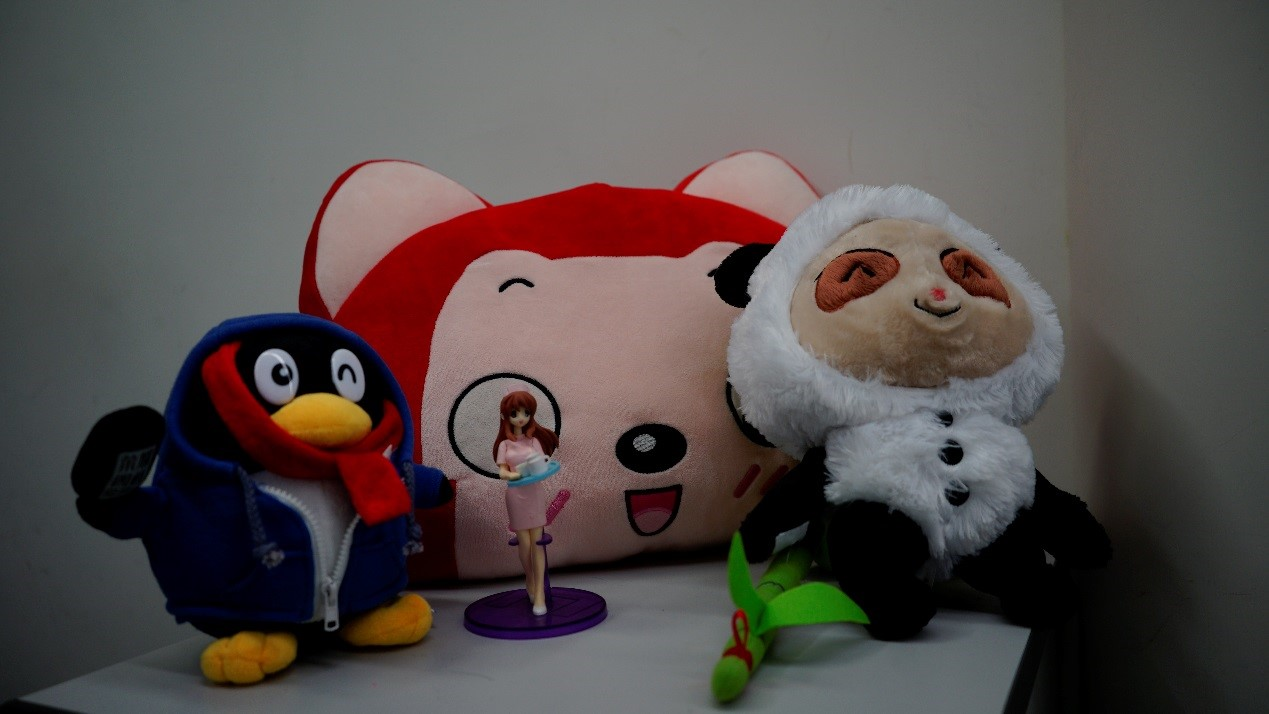
\includegraphics[width=1\textwidth]{images/dataset/200_3-5_1-60.jpg}
	   \caption{200,3.5,1/60}
    \end{subfigure}
    \hfill
    \begin{subfigure}[t]{0.32\textwidth}
        \centering
        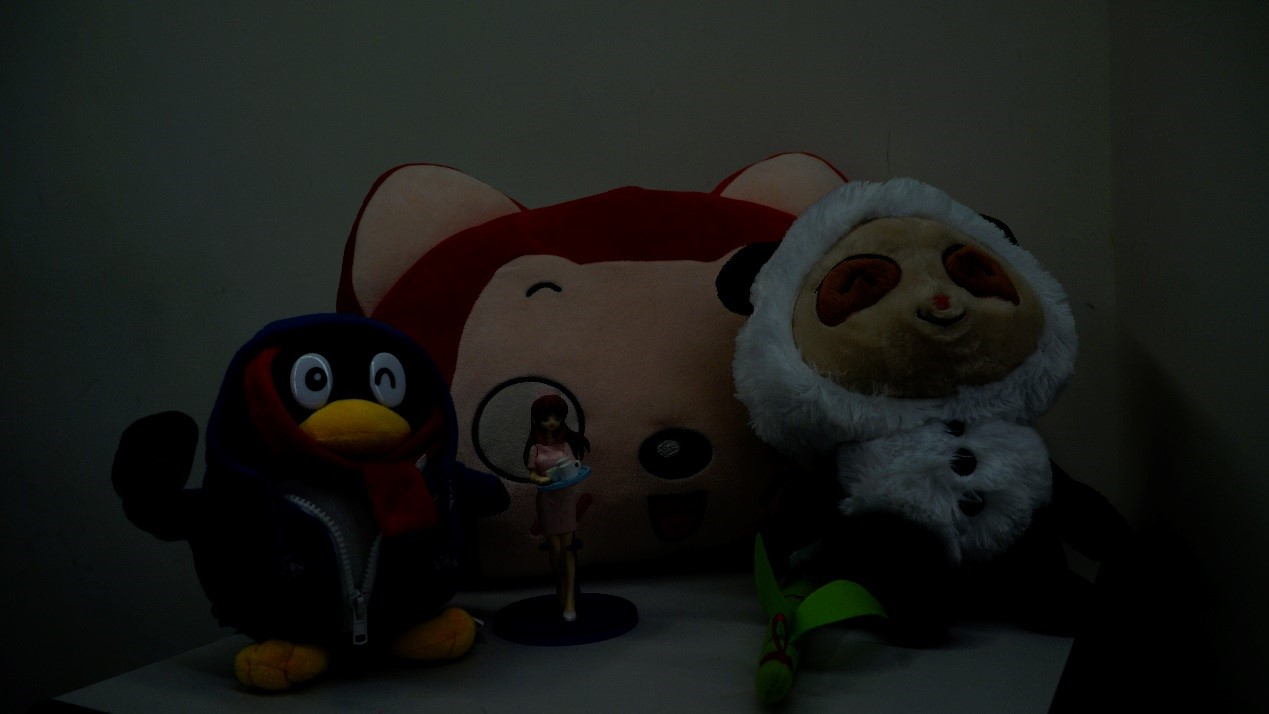
\includegraphics[width=1\textwidth]{images/dataset/200_6-7_1-60.jpg}
		\caption{200,6.7,1/60}
    \end{subfigure}
    \hfill
    \begin{subfigure}[t]{0.32\textwidth}
        \centering
        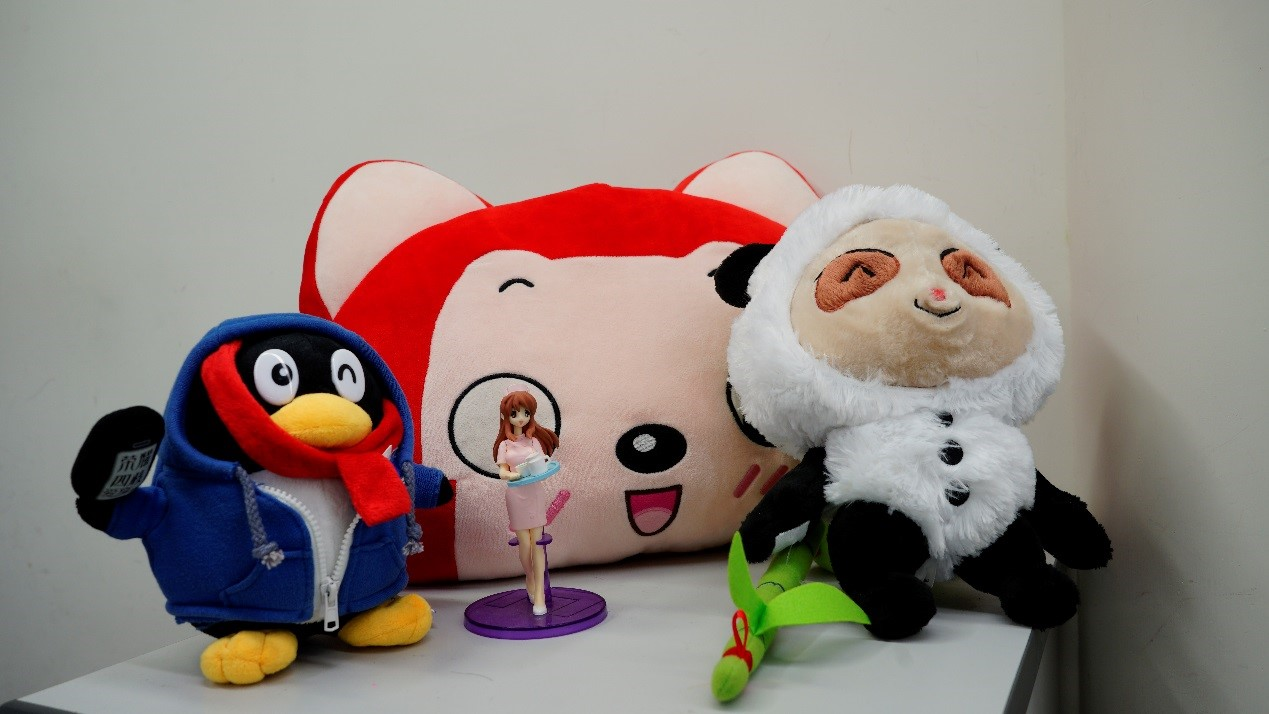
\includegraphics[width=1\textwidth]{images/dataset/200_6-7_1-8.jpg}
		\caption{200,6.7,1/8}
    \end{subfigure}
    \hfill
    \begin{subfigure}[t]{0.32\textwidth}
        \centering
        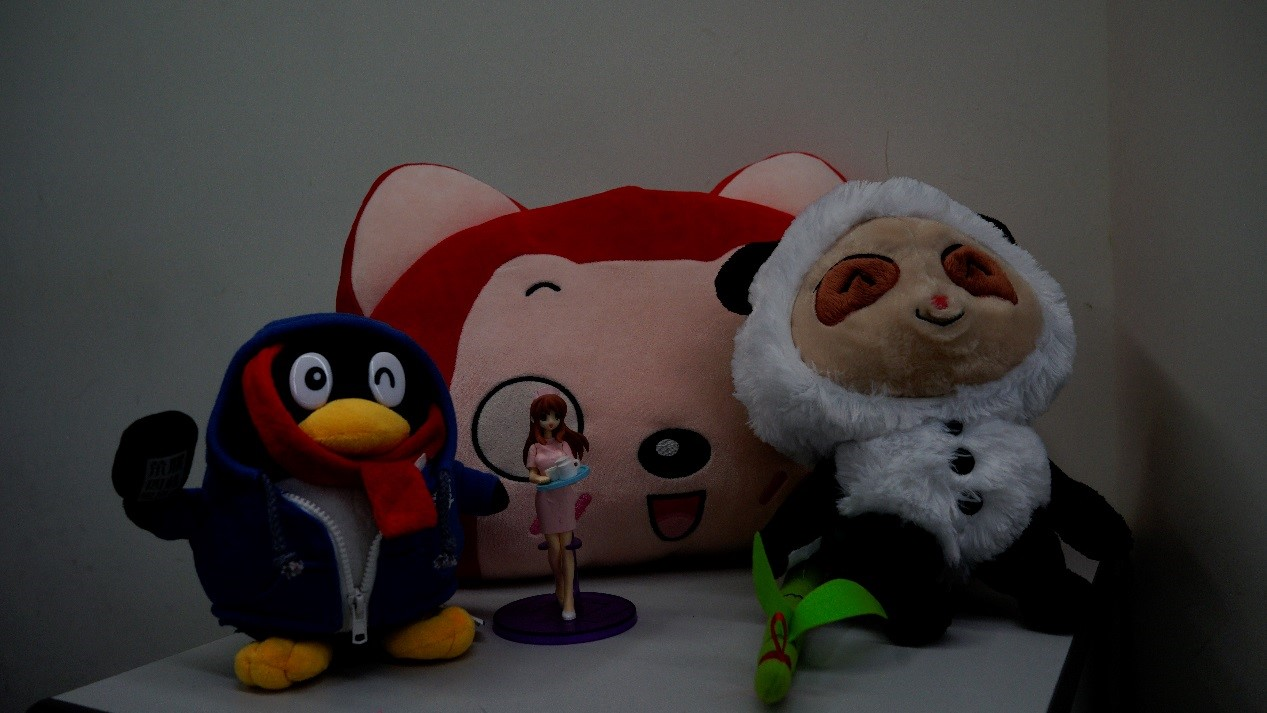
\includegraphics[width=1\textwidth]{images/dataset/400_6-7_1-60.jpg}
		\caption{400,6.7,1/60}
    \end{subfigure}
    \hfill
    \begin{subfigure}[t]{0.32\textwidth}
        \centering
        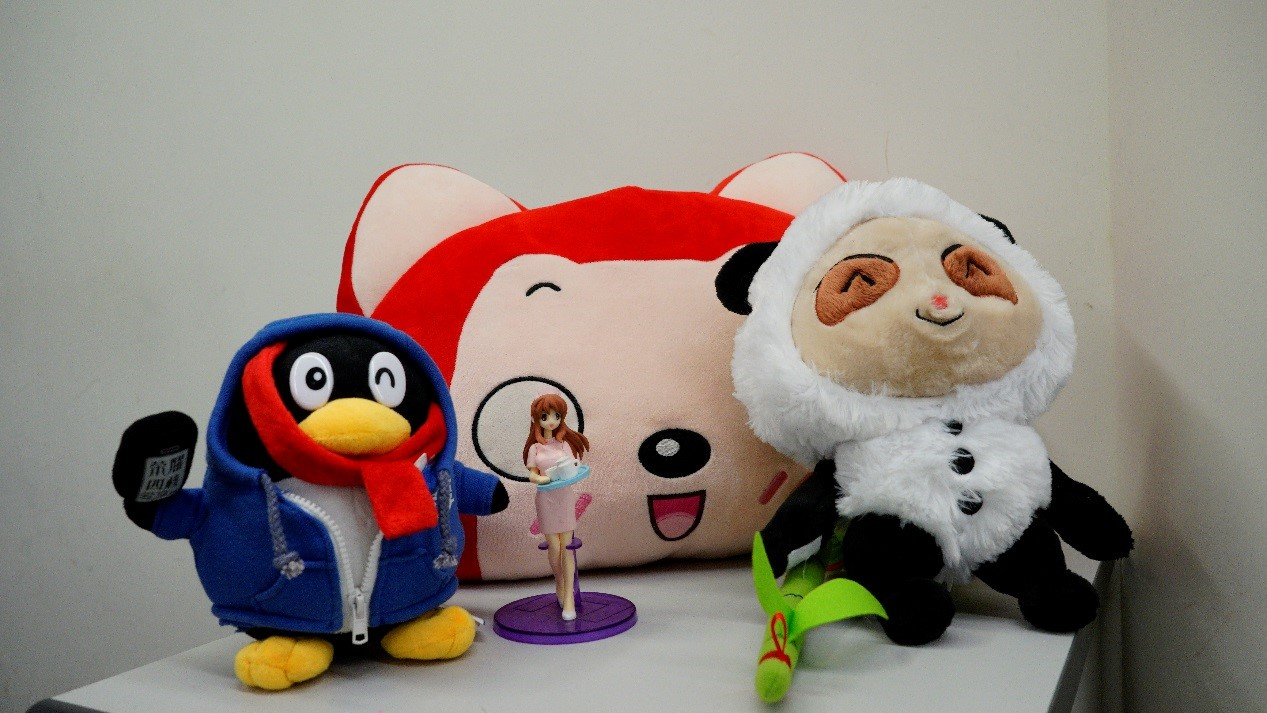
\includegraphics[width=1\textwidth]{images/dataset/1600_6-7_1-60.jpg}
		\caption{1600,6.7,1/60}
    \end{subfigure}
    \hfill
    \begin{subfigure}[t]{0.32\textwidth}
        \centering
        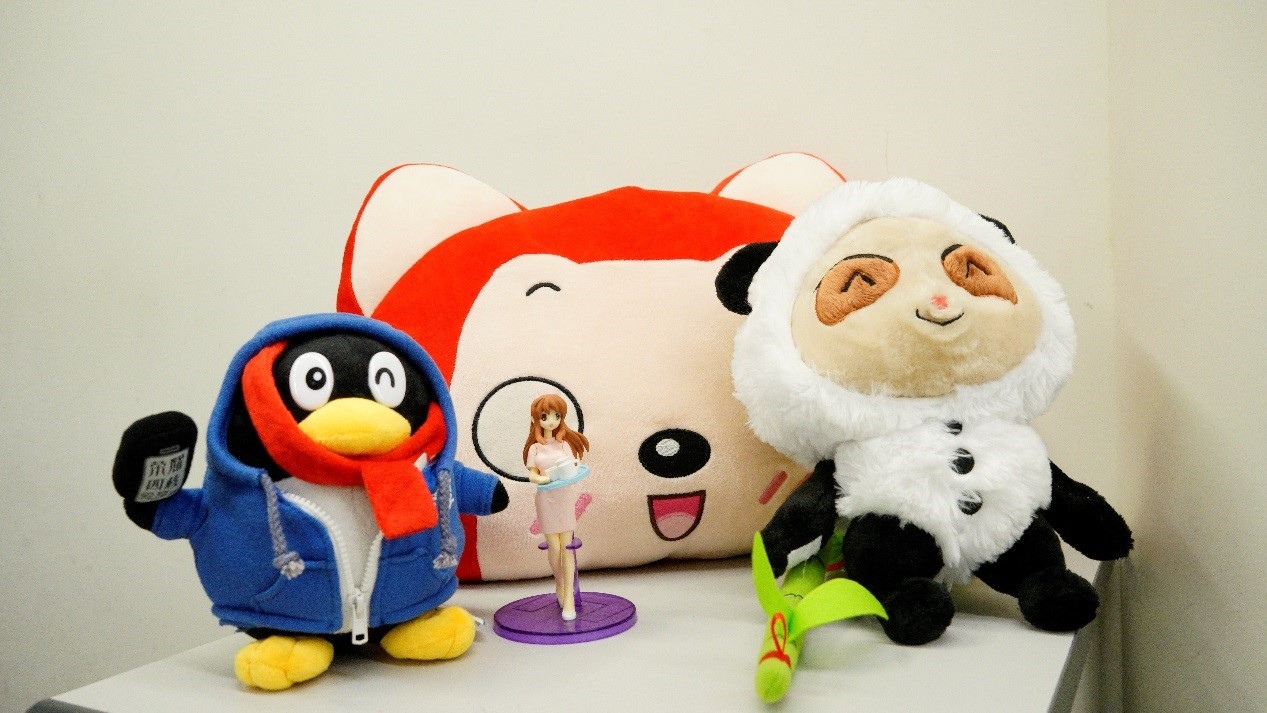
\includegraphics[width=1\textwidth]{images/dataset/3200_6-7_1-60.jpg}
		\caption{3200,6.7,1/60}
    \end{subfigure}
    \hfill
    \begin{subfigure}[t]{0.32\textwidth}
        \centering
        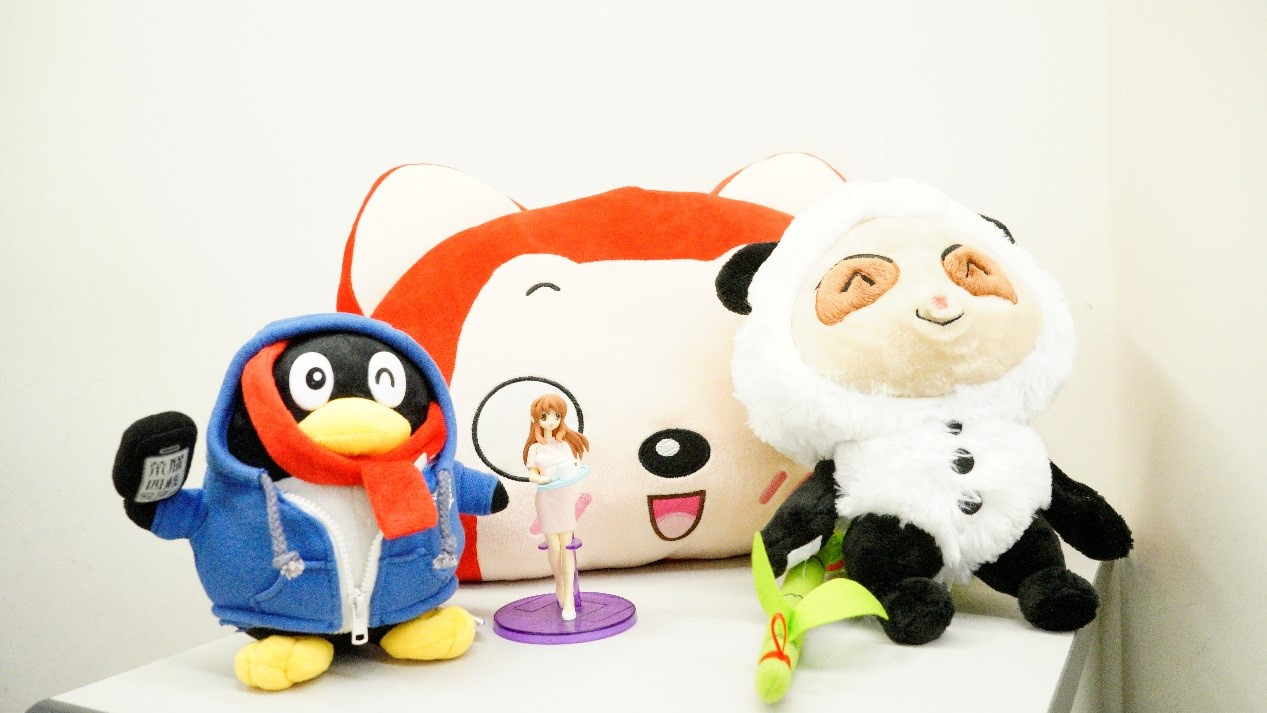
\includegraphics[width=1\textwidth]{images/dataset/6400_6-7_1-60.jpg}
		\caption{6400,6.7,1/60}
    \end{subfigure}
    \hfill
    \begin{subfigure}[t]{0.32\textwidth}
        \centering
        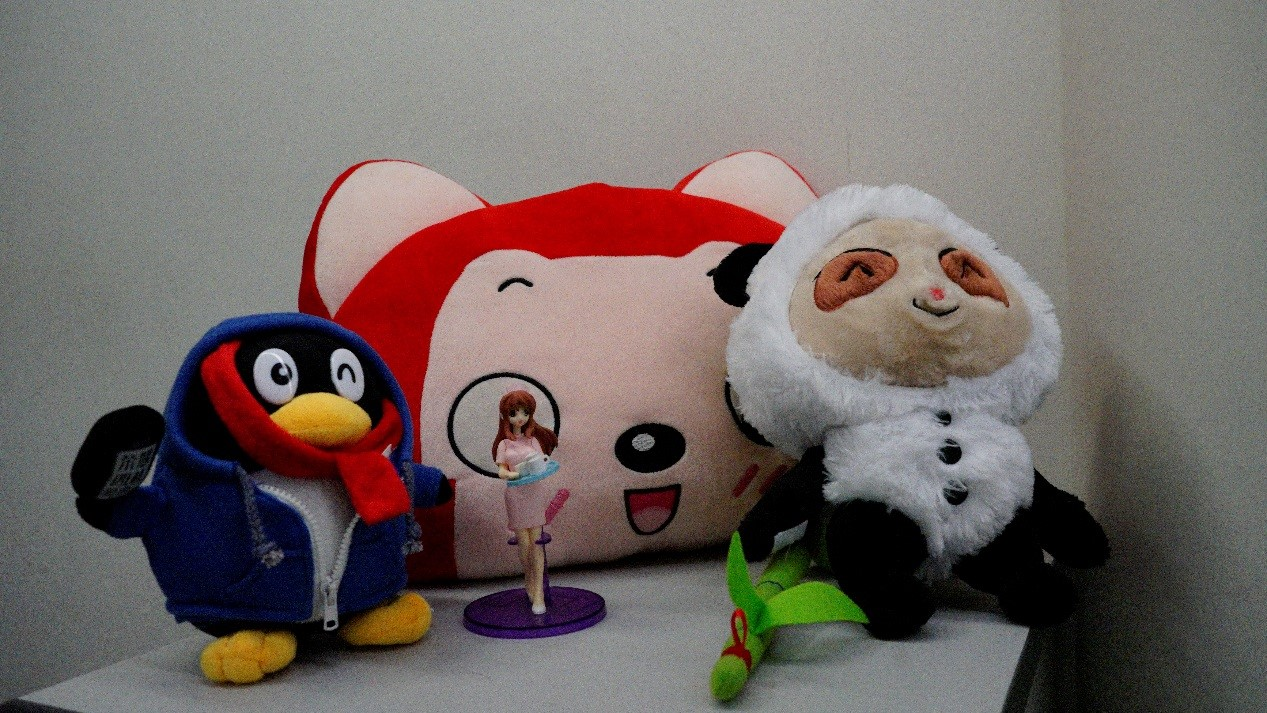
\includegraphics[width=1\textwidth]{images/dataset/6400_6-7_1-350.jpg}
		\caption{6400,6.7,1/350}
    \end{subfigure}
    \hfill
    \begin{subfigure}[t]{0.32\textwidth}
        \centering
        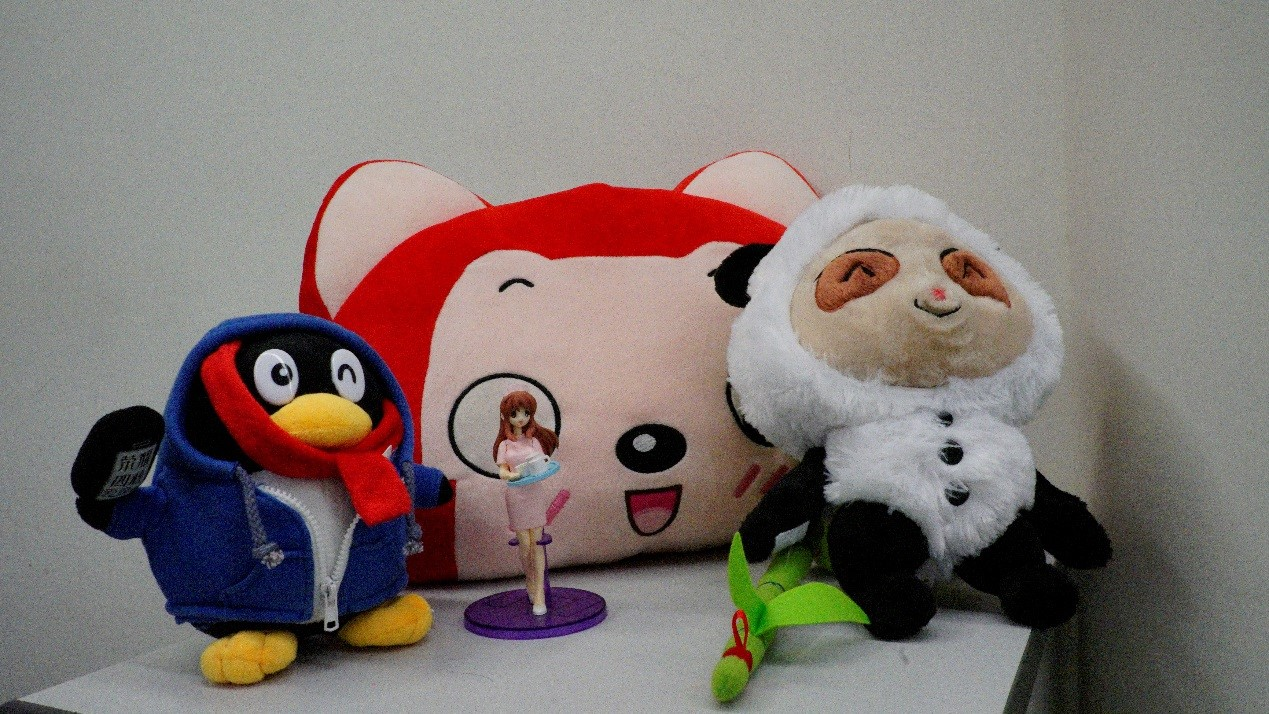
\includegraphics[width=1\textwidth]{images/dataset/6400_16_1-60.jpg}
		\caption{6400,16,1/60}
    \end{subfigure}
    \caption{Captured Images with the Sony A7 II camera under different (ISO, Shutter, Aperture) settings.}
    \label{fig6}
\end{figure}


\section{Analysis and Discussion}


\section{Experiments}










\section{Conclusion}